\begin{flushleft}
{\bf Появление отдельных сумм очков при 36 бросаниях двух кубиков.} 
\end{flushleft}

\begin{flushright}
Таблица 3
\end{flushright}

\begin{center}
\begin{tabularx}{\textwidth}{| c | X | X | X | X | X | X | X | X | X | X | X |}
\hline
$\sum$ & 2 & 3 & 4 & 5 & 6 & 7 & 8 & 9 & 10 & 11 & 12 \\ \hline
{\bf к р а т н о с т ь} & 1 & 2 & 2 & 6 & 3 & 5 & 4 & 7 & 1 & 3 & 2 \\ \hline
\end{tabularx}


\end{center}
 

\begin{flushleft}
{\bf Сумма очков на костях при всех возможных исходах бросания двух кубиков.}
\end{flushleft}

\begin{center}
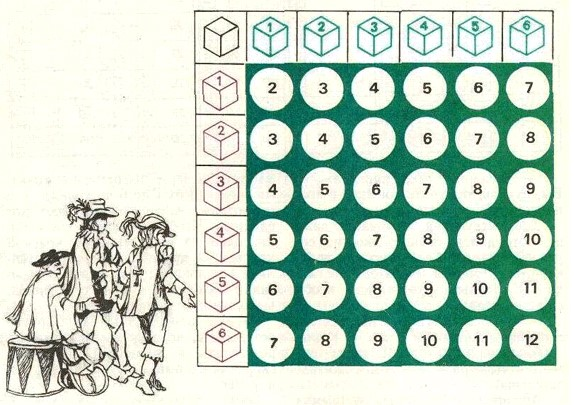
\includegraphics[scale=0.9]{img.jpg}
\end{center}

\begin{multicols}{2}
\noindent
отличаться от 1/6 (среднего значения) частоты выпадений различных очков от 1 до 6. Можно сказать, что выпадение любого из шести очков при бросании симметричной кости равновероятно. А вот появление разных значений сумм очков при бросании двух костей оказывается не равновероятным.

\noindent
Можете ли вы сказать почему?

\noindent
Давайте составим таблицу всех возможных исходов при бросании красной и синей костей. Так как выпадение любого числа очков от 1 до 6 на красной кости может сочетаться с любым числом очков на синей кости, то у нас получится таблица 4.

\noindent
Любое из 36 сочетаний очков на красной и синей костях равновероятно любому другому сочетанию, но разные суммы очков могут быть получены различным числом способов. Так, сумма очков 3 (у Д'Артаньяна) получается двумя способами 1 + 2 и 2 + 1, а сумма 2 (у англичанина) --- лишь одним (из 36!): 1 + 1. Атосу было чему удивляться!

\noindent
{\bf Вероятность}

\noindent
Вы видите, что выпадение 2 и 6 очков на одной кости равновероятны, а выпадение суммы 2 и 7 на двух костях не равновероятны. В подобных случаях говорят, что сумме 7 {\it благоприятствует} больше исходов из общего числа равновероятных исходов, чем сумме 2. Так, сумме 7 благоприятствуют шесть исходов из общего числа равновероятных исходов, равного 36, тогда как суммк 2 благоприятствует лишь один исход.

\noindent
И в общем случае подсчёт числа благоприятных исходов из их общего числа - важнейшее действие для определения в е р о я т н о с т и события, под которой понимают {\it отношение числа благоприятных исходов к общему числу равновероятных исходов}. При этом используется такие обозначения. Само событие (например, появление суммы 7) обозначается буквой А, а вероятность этого события --- {\it P(A)}. Итак,
\begin{equation*}
P(A)=\frac{m}{n},
\end{equation*}
\end{multicols}


\begin{flushright}
{\bf (*)}
\end{flushright}

